\subsubsection{\Glspl{bearing-angle-image}}

\begin{figure}[H]
    \centering
    \tikzset{every picture/.style={line width=0.75pt}} %set default line width to 0.75pt        

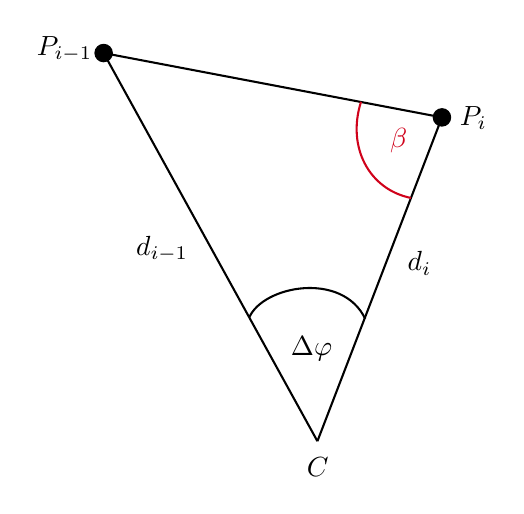
\begin{tikzpicture}[x=0.75pt,y=0.75pt,yscale=-1,xscale=1]
%uncomment if require: \path (0,227.75); %set diagram left start at 0, and has height of 227.75

%Straight Lines [id:da05017383740499093] 
\draw    (38.83,15.67) -- (141.83,202.67) ;


%Straight Lines [id:da6895513561877372] 
\draw    (201.83,46.67) -- (141.83,202.67) ;


%Curve Lines [id:da10253757735662583] 
\draw [color={rgb, 255:red, 0; green, 0; blue, 0 }  ,draw opacity=1 ]   (109,143) .. controls (115.83,127.67) and (153.83,120.67) .. (164.83,143.67) ;


%Straight Lines [id:da3851492122035306] 
\draw    (38.83,15.67) -- (201.83,46.67) ;


%Curve Lines [id:da7052636563383052] 
\draw [color={rgb, 255:red, 208; green, 2; blue, 27 }  ,draw opacity=1 ]   (162.83,39.17) .. controls (155.83,61.17) and (166.9,81.48) .. (186.9,85.48) ;


%Shape: Circle [id:dp08101382020617043] 
\draw  [fill={rgb, 255:red, 0; green, 0; blue, 0 }  ,fill opacity=1 ] (197.88,46.67) .. controls (197.88,44.49) and (199.65,42.72) .. (201.83,42.72) .. controls (204.01,42.72) and (205.78,44.49) .. (205.78,46.67) .. controls (205.78,48.85) and (204.01,50.62) .. (201.83,50.62) .. controls (199.65,50.62) and (197.88,48.85) .. (197.88,46.67) -- cycle ;
%Shape: Circle [id:dp7397482298206297] 
\draw  [fill={rgb, 255:red, 0; green, 0; blue, 0 }  ,fill opacity=1 ] (34.88,15.67) .. controls (34.88,13.49) and (36.65,11.72) .. (38.83,11.72) .. controls (41.01,11.72) and (42.78,13.49) .. (42.78,15.67) .. controls (42.78,17.85) and (41.01,19.62) .. (38.83,19.62) .. controls (36.65,19.62) and (34.88,17.85) .. (34.88,15.67) -- cycle ;


% Text Node
\draw (139,158) node [color={rgb, 255:red, 0; green, 0; blue, 0 }  ,opacity=1 ] [align=left] {$\displaystyle \Delta $$\displaystyle \varphi $};
% Text Node
\draw (181,58) node [color={rgb, 255:red, 208; green, 2; blue, 27 }  ,opacity=1 ] [align=left] {$\displaystyle \beta $};
% Text Node
\draw (191,117) node  [align=left] {$\displaystyle d_{i}$};
% Text Node
\draw (67,110) node  [align=left] {$\displaystyle d_{i-1}$};
% Text Node
\draw (217,47) node  [align=left] {$\displaystyle P_{i}$};
% Text Node
\draw (20,14) node  [align=left] {$\displaystyle P_{i-1}$};
% Text Node
\draw (142,215) node  [align=left] {$\displaystyle C$};


\end{tikzpicture}
%
    \caption[Schematic Representation of Bearing-Angles]{This figure shows the relationship of the light rays that form the \gls{bearing-angle}.}
\end{figure}

Existing literature\cite{Scaramuzza2007,Lin2017} proposes \Glspl{bearing-angle-image} were each pixel is the angle between the current point, the optical center and the previous point.
The neighbourhood relationship can be choosen arbitrarily resulting in four first-order \Glspl{bearing-angle-image}, horizontal, vertical, diagonal and antidiagonal.
The second variable is the direction the angle is calculted, e.g.~for horizontal images it can be calculated from left-to-right or right-to-left.
This does not exhibit new information, because the angle of the other direction is immediatly known from the fact that the sum of the angles is $180\degree$.
Nontheless, the direction must be defined to obtain stable visual features.

The formula for the \gls{bearing-angle} $\beta$ is derived with the cosine theorem.
For the horizontal left-to-right calculation the formula is as follows.
\begin{equation}
    \beta = \arccos%
            \frac{d_{i,j} - d_{i-1,j} \cos \Delta\varphi}%
                 {\sqrt{d_{i,j}^2 + d_{i-1,j}^2 - 2 d_{i,j} d_{i-1,j} \cos \Delta\varphi}}
\end{equation}
Using a different direction or other neighbourhood relation the indices for the depth values need to be changed and a different angular resolution needs to be calculated.
The \Gls{bearing-angle} is in the range $\beta \in (0, \pi)~rad$.
Linear scaling of the angle to the color depth of the target image results in a grayscale image suitable for feature extraction.
A general scaling function for an $unsigned~8bit$ image and arbitrary angle range follows here.
This formulation can be used for different color depths and other potential angle calculations that result in different boundary conditions.
\begin{equation}
\begin{aligned}
    \beta_{min} &= 0 ~& c_{min} &= 0 \\
    \beta_{max} &= \pi ~& c_{max} &= 255 \\
    \beta_{scaled} &= \floor*{c_{min} + \beta \frac{c_{max} - c_{min}}{\beta_{max} - \beta_{min}}}
\end{aligned}
\end{equation}
